Plugin del browser Google Chrome, che permette di navigare il sito dal punto di vista di una persona affetta da una certa disabilità visiva.\\
\begin{itemize}
	\item Può simulare uno screen reader, in modo da poter capire se il sito è accessibile o meno.
	\item Può simulare la visualizzazione del sito da parte di una persona miope, con parziale cecità oppure dislessia.
	\item Può simulare la visualizzazione del sito da parte di una persona che soffre di daltonismo, ovvero che ha un'alterata percezione dei colori.
\end{itemize}
L'obiettivo è rendere accessibile il sito a più categorie di utenti possibili. Purtroppo la grande quantità di problemi e disturbi rendono arduo l'obiettivo di raggiungere tutti gli utenti, ma questi strumenti aiutano a perfezionare i dettagli, che agli sviluppatori possono sfuggire nella codifica incrementale del sito.
\begin{figure}[!h]
	\centering
	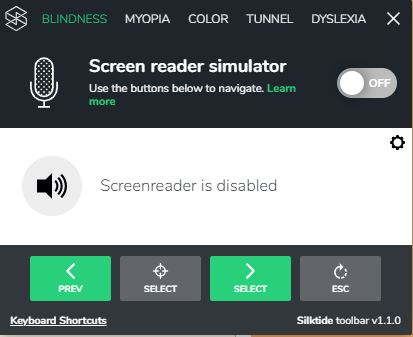
\includegraphics[width=0.7\linewidth]{sezioni/FaseTest/Immagini/screen_reader_simulator.JPG}\\
	\caption{Silktide – disability simulator : screen reader simulator}
	\label{Fig:silktide}
\end{figure} 